
\documentclass[a4paper,graphics,11pt]{article}

\usepackage[utf8]{inputenc}
\usepackage[T1]{fontenc}
\usepackage{lmodern}
\usepackage[ngerman]{babel}
\usepackage{amsmath, tabu}
\usepackage{amsthm}
\usepackage{amssymb}
\usepackage{algorithm}
\usepackage{algpseudocode}
\usepackage{mathtools}
\usepackage{setspace}
\usepackage{graphicx,color,curves,epsf,float,rotating}
\usepackage{eurosym}
\usepackage{tikz}
\usepackage{../tikz-uml}
\usepackage{listings}

\floatname{algorithm}{Algorithmus}

\newcommand\norm[1]{\left\lVert#1\right\rVert}
\newcommand\abs[1]{\left\vert#1\right\vert}

\newcommand\aufgabe[1]{\subsection*{Aufgabe #1}}
\newcommand\aufgabenteil[1]{\subsubsection*{#1}}



\pagestyle{empty}
\begin{document}
\noindent WS 2016/17                      \hfill Simon Kaiser, 354692 \\
\null                                     \hfill Philipp Hochmann, 356148 \\
\null                                     \hfill Felix Kiunke, 357322 \\
\null                                     \hfill Giacomo Klingen, 356778 \\
\null                                     \hfill Daniel Schleiz, 356092 \\

\begin{center}
\Large \textsc{Softwaretechnik} \\   % Fach
\large Aufgabenblatt 8               % Nummer das Blattes
\end{center}
\begin{center}
\rule[0.5ex]{\textwidth}{0.6pt}\vspace*{-\baselineskip}\vspace{3.2pt}
\rule[0.5ex]{\textwidth}{1.6pt}\\
\end{center}


%%%%%%%%%%%%%%%%%%%%%%%%%%%%%%%%%%%%%%
%
%   Ab hier kommt der Text
%   Neue Aufgabe mit \aufgabe{}
%   Aufgabenteil mit \aufgabenteil{}
% 
%%%%%%%%%%%%%%%%%%%%%%%%%%%%%%%%%%%%%%

\aufgabe{8.1}
Man trennt die Software-Produktlinie in zwei Bereiche, welche abhängig voneinander entwickelt werden.\\

Die erste Phase wird als \textit{Domänen Engineering} bezeichnet. Man erfasst alle relevanten Konzepte der Domäne, aus der 
man die Realisierung einer wiederverwendbaren Plattform produziert. (Man muss sowohl die Gemeinsamkeiten als auch die 
Unterschiede der einzelnen Produkte einbauen.) Durch die Wiederverwendung der Komponenten spart man bei den
Produktionskosten und trägt zu einer besseren Qualität der Komponenten bei.\\

Um die Endprodukte zugeschnitten auf die Bedürfnisse der einzelnen Kunden zu entwickeln, 
werden in dem zweiten Bereich, das \textit{Applikation Engineering}, die wiederverwendbaren Komponenten der Plattform 
ausgewählt und miteinander integriert. Dabei wird mit dem Domänen Engineering insofern zusammengearbeitet, 
dass wiederverwendbare Komponenten bestimmt werden.

\aufgabe{8.2}
\begin{tikzpicture}

\umlstateinitial[name=start,anchor=south west,x=0,y=0]

\umlbasicstate[name=standby,x=1,anchor=west,y=0]{Standby}

\umlbasicstate[name=play,anchor=west,y=-5]{Nachrichten abspielen}

\umltrans{start}{standby}

\umltrans[recursive=70|110|1cm,recursive direction=top to top,arg={WD[KN]/},
	pos=2]{standby}{standby}

\umlHVtrans[arg={WD[EN]/},anchor1=210,anchor2=140,pos=1.45,align=right]{standby}{play}
\umlHVtrans[arg={NA},anchor1=210,anchor2=140,pos=1.55,align=right]{standby}{play}
\umltrans[arg={SD/WS},anchor1=50,anchor2=-110,align=right,pos=0.2]{play}{standby}
\umltrans[arg={[AN]/WS},anchor1=35,anchor2=-78,align=left,pos=0.2]{play}{standby}

\begin{umlstate}[name=call,x=7,y=-1]{Anruf}
	\umlstateinitial[anchor=south west,name=cstart]
	\umlbasicstate[name=cva,x=4]{Verbindungsaufbau}
	\umlbasicstate[name=ca,y=-3]{Aufnahme}
	\umlstatefinal[anchor=south east,name=end,x=5,y=-3]

	\umltrans{cstart}{cva}
	\umlVHVtrans[anchor1=-130,anchor2=90,arm1=-0.2,arg={[cmax]/A1,AS},pos=2.3]
		{cva}{ca}
	\umltrans[arg={AL/UT},pos=0.5,anchor1=3]{ca}{end}
	\umltrans[anchor1=-56,arg={[=max]/A2,UT},align=right,pos=0.9]{cva}{end}
\end{umlstate}

\umlHVHtrans[anchor1=200,anchor2=-30,arm1=-3,arg={AL/VT},pos=2.27,align=right]
	{cva}{standby}
\umltrans[anchor1=9,anchor2=148,arg={AK/AA},pos=0.5]{standby}{call}

\end{tikzpicture}


\aufgabe{8.3}
\aufgabenteil{a)}
Die Idee hinter der Code-Generierung ist, durch das automatisierte Generieren von Programmcode(teilen) aus
einer Modellsprache sowohl Zeit einzusparen als auch eine höhere Qualität in Hinblick auf die Strukturierung und Lesbarkeit zu erzielen.

\aufgabenteil{b)}
%%%%%%%%%%%%%%%%%%%%%%%%%%%%%%%%%%%%%%%%
%% Klassendiagramm, evtl. texen       %%

\begin{figure}[h]
  \centering
  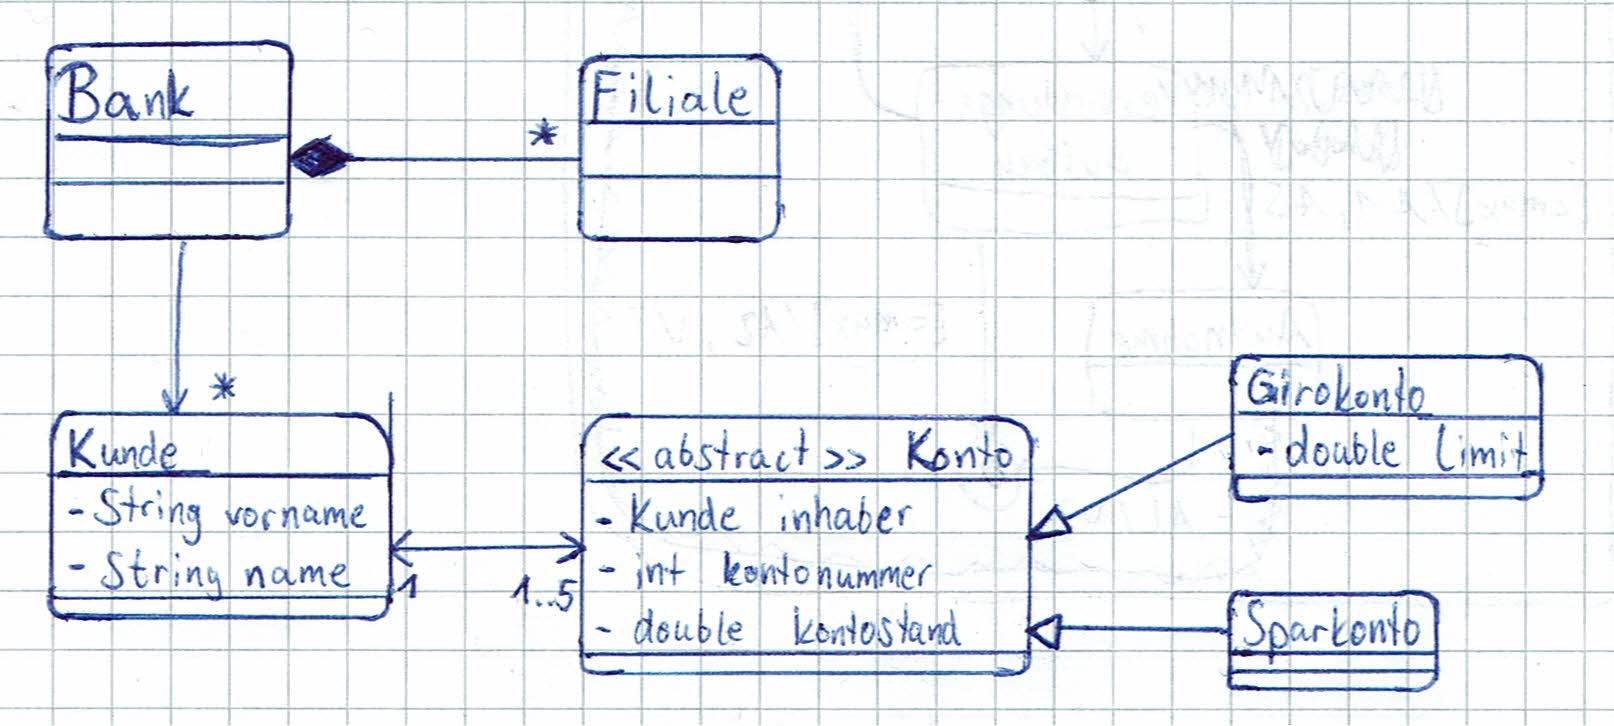
\includegraphics{3b_classdiag}
\end{figure}

%%                                    %%
%%%%%%%%%%%%%%%%%%%%%%%%%%%%%%%%%%%%%%%%

\lstset{
    %basicstyle=\ttfamily,
    keywordstyle=\bfseries,
    showstringspaces=false,
    morekeywords={classdiagram, class, abstract, extends, association}
}
\begin{minipage}{\linewidth}
Nun folgt die textuelle Beschreibung der geforderten Elemente des Klassendiagramms:\\
\begin{lstlisting}
classdiagram BankSystem {
    class Kunde {
       String vorname;
       String name;
    }
    abstract class Konto {
       Kunde inhaber;
       int kontonummer;
       double kontostand;
    }
    class Girokonto extends Konto {
       double limit;
    }
    association [1] Kunde <-> Konto [1..5];
}
\end{lstlisting}
\end{minipage}

\end{document}
